\documentclass[10pt]{scrartcl}

\usepackage[utf8]{inputenc}
\usepackage{tabularx}
\usepackage{longtable}
\usepackage[ngerman]{babel}
\usepackage[automark]{scrpage2}
\usepackage{amsmath,amssymb,amstext}
%\usepackage{mathtools}
\usepackage[]{color}
\usepackage[]{enumerate}
\usepackage{graphicx}
\usepackage{lastpage}
\usepackage[perpage,para,symbol*]{footmisc}
\usepackage{listings} 
\usepackage[pdfborder={0 0 0},colorlinks=false]{hyperref}
\usepackage[numbers,square]{natbib}
\usepackage{color}
\usepackage{colortbl}
\usepackage[absolute]{textpos}
\usepackage{float}
\usepackage[colorinlistoftodos,textsize=small,textwidth=2cm,shadow,bordercolor=black,backgroundcolor={red!100!green!33},linecolor=black]{todonotes}

\lstset{numbers=left, numberstyle=\tiny, numbersep=5pt, breaklines=true, showstringspaces=false} 
\restylefloat{figure}

%changehere
\def\titletext{Lab 2: SIP, Multicast}
\def\titletextshort{Praktikum 2}
\author{André Harms, Oliver Steenbuck}

\title{\titletext}

%changehere Datum der Übung
\date{04.01.2012}

\pagestyle{scrheadings}
%changehere
\ihead{TT1, Schmidt}
\ifoot{Generiert am:\\ \today}

\cfoot{Oliver Steenbuck, André Harms}


\ohead[]{\titletextshort}
\ofoot[]{{\thepage} / \pageref{LastPage}}

\setlength{\parindent}{0.0in}
\setlength{\parskip}{0.1in}

\begin{document}
\maketitle

\setcounter{tocdepth}{3}
\tableofcontents

%	\listoftables                                 												% 
%	\listoffigures   

\section{Durchführung des Versuchs}
Beim Testen der Anwendung, um einen Dump der Netzwerkkommunikation zu erhalten, wurde die Anwendung am SIP-Proxy registriert und von zwei Clients angerufen (invited). Anschließend haben die Clients nacheinander mittels eines Byes die Verbindung beendet. Dieses Vorgehen und der Multicastverkehr wurden aufgezeichnet.
	
\section{Beobachtung}

\section{Bedienung der Anwendung}
\begin{enumerate}
	\item entpacken \verb!harmsSteenbuckSIP.tgz!
	\item wechseln in das Verzeichnis \verb!dist!
	\item \verb!java -jar "SIPGUI.jar"!
	\item Die unter \ref{sec:bedienung:anwendung} beschrieben Anwendung startet
\end{enumerate}

\section{Bedienung der Anwendung}
\label{sec:bedienung:anwendung}		
	\begin{figure}[H]
        \centering
                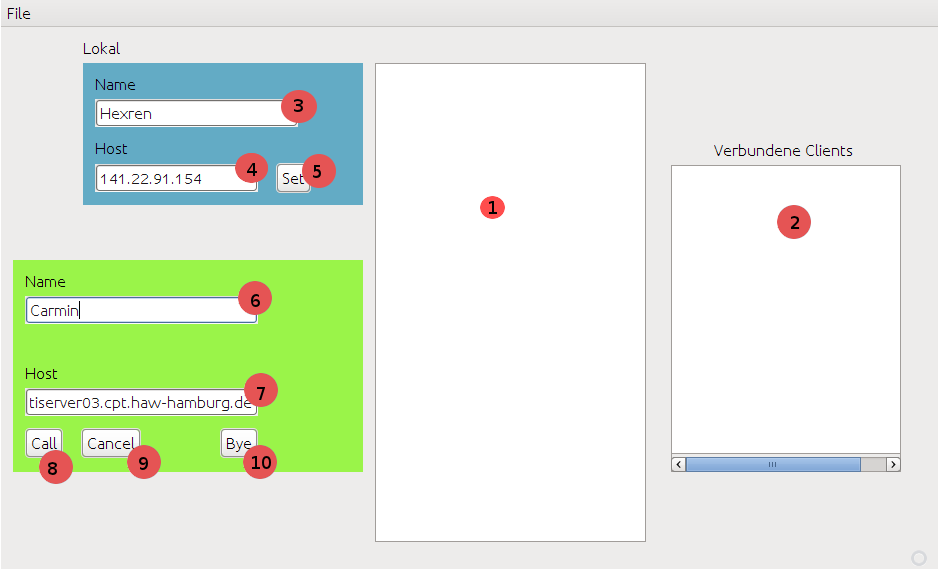
\includegraphics[width=\textwidth]{img/screenshotApplication}
        \caption{Screenshot der GUI}
        \label{img:gui}
	\end{figure}

\begin{enumerate}
	\item Bereich in dem die empfangenen IGMP Nachrichten angezeigt werden
	\item Zum Server verbundene Clients
	\item Name mit dem sich beim Proxy registriert wird
	\item IP Adresse des Rechners
	\item Knopf zum Registrieren
	\item Name des zu invitenden Teilnehmers
	\item IP Adresse des zu invitenden Teilnehmers
	\item Knopf zum Anrufen (inviten) des in X angegebenen Teilnehmers
	\item Knopf zum Abbrechen eines Invites
	\item Knopf zum Beenden der Verbindung
\end{enumerate}

\section{Sourcen}
Das Project besteht im wesentlichen asu 2 teilen. Zum ersten eine Bibliothekt die SIP und IGMP funktionalitäten bietet und in Eclipse mit Maven entwickelt wurde zum anderene ine Oberfläche die in Netbeans entwickelt wurde und die Bibliothek nutzt.

Die Sourcen für beide Projekte sind auf githup unter folgenden Pfaden verfügbar.
\begin{description}
	\item[Bibliothek] Eclipse \\ \verb!https://github.com/MyersGer/WS_2011/tree/master/TT1/Prak2/lab3!
	\item[Oberfläche] Netbeans \\ \verb!https://github.com/MyersGer/WS_2011/tree/master/TT1/Prak2/guiHarmsSteenbuck!
\end{description}

\section{Anlagen}
\begin{itemize}
	\item ausführbare Jar
\end{itemize}

\end{document}

